
	\subsection{2.16. Диаграммы МО для электроноизбыточных соединений.} 
	
	\par\bigskip
	
	\begin{figure}[H]
		\centering
		{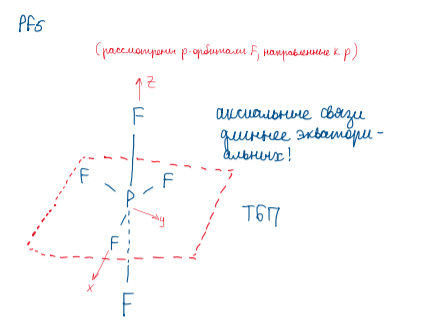
\includegraphics[scale=1]{44.png}}
	\end{figure}
	
	\begin{figure}[h]
		\centering
		{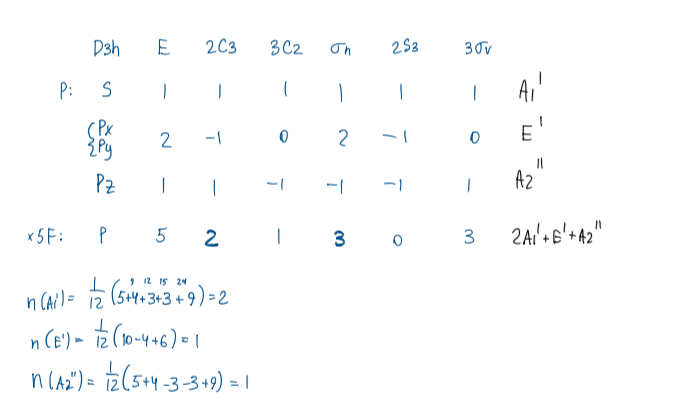
\includegraphics[scale=1]{45.png}}
	\end{figure}
	
		\begin{figure}[H]
		\centering
		{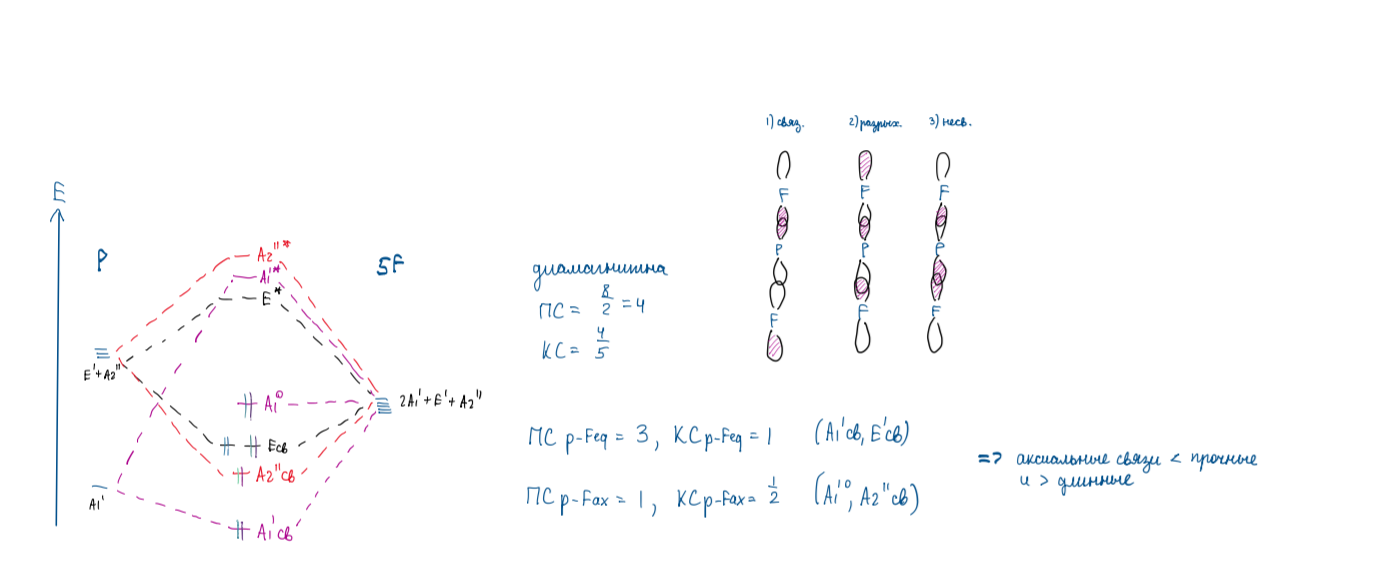
\includegraphics[scale=0.7]{46.png}}
	\end{figure}

	\begin{figure}[H]
	\centering
	{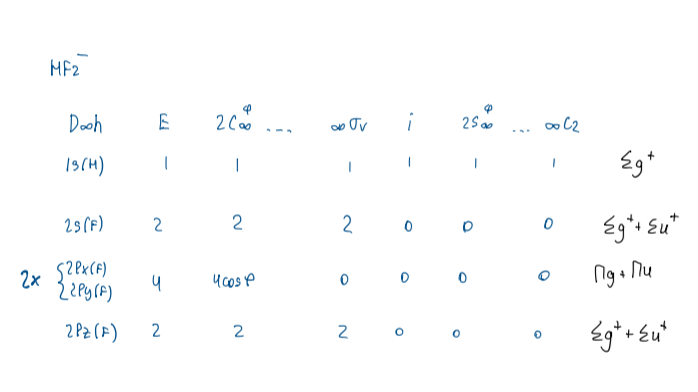
\includegraphics[scale=1]{47.png}}
\end{figure}

	\begin{figure}[H]
	\centering
	{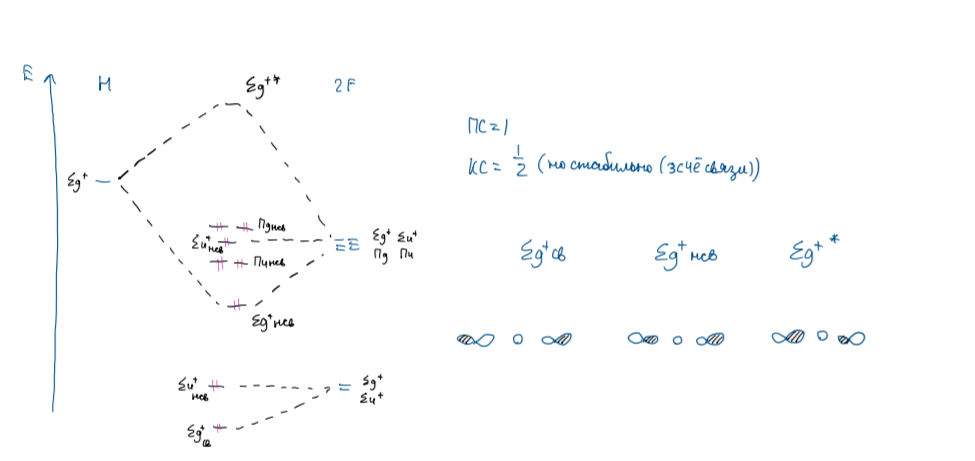
\includegraphics[scale=0.7]{48.png}}
\end{figure}
	
	
	Лучше всего такие электроноизбыточные рассматривать с позиций метода молекулярных орбиталей. Молекула $PCl_5$ ($PF_5$ тоже) представляет собой тригональную бипирамиду. Из геометрии понятно, что,
	вообще говоря, атомы фтора не эквивалентны друг другу, ведь есть три экваториальных атома и два аксиальных атома фтора. Более того, расстояния фосфор-аксиальный фтор больше, чем фосфорэкваториальный фтор. Кстати, так как молекулы колеблятся, то положение плоскости может измениться, и аксиальные атомы перейдут в экваториальные, или наоборот. Это псевдопревращения Берри. Из-за
	колебательных процессов, реально атомы усредняются и становятся одинаковыми.
	
	\par\smallskip
	
	Если рассмотреть взаимодействие фосфора с тремя экваториальными атомами фтора, то видно, что у каждого фтора становится по 8 электронов, а у фосфора остаётся ещё одна pz-орбиталь и ещё два своих
	электрона. На оставшуюся систему из фосфора и двух аксиальных атомов фтора приходится 3 орбитали и 4 электрона. Понятно, что существует только три комбинации перекрытия трёх орбиталей. Это
	связывающая и разрыхляющая орбитали, но есть ещё несвязывающая орбиталь. Получается, что из симметрии «место» для такой орбитали в молекуле нашлось, и молекула может удерживать там электроны,
	хоть они и не вносят никакого вклада в связывание - «сколько выиграли, столько и проиграли». Так как 3 атома удерживаются только 2 электронами (на связывающей орбитали), то связь длиннее. В итоге
	имеем, что у атома фосфора недостаточно орбиталей. Поэтому такие соединения называются орбитальнодефицитными электроноизбыточными.
	
	\par\smallskip
	
	Заметим, что три комбинации перекрывания орбиталей существует и для центральных атомов с s-орбиталью, например, в $HF_2^-$. Это очень устойчивый молекулярный ион, хоть у водорода 4 электрона (правило
	инертного газа для него - 2 электрона). Есть гексафторсиликат-ион (октаэдрическое строение), там имеется три (по каждой оси) таких 3с4е-взаимодействия.
	
	\par\smallskip
	
	Из вышеперечисленных особенностей электронного строения следуют некоторые химические особенности. Такие молекулы являются основаниями Льюиса, то есть, донорами электронной пары. Во-первых,
	если молекула отдаст электронную пару с несвязывающей орбитали, порядок её связывания не изменится. Во-вторых, если у молекулы было 10 электронов (тот же $PF_5$), то в результате образуется очень
	устойчивая восьмиэлектронная система. 
	
	
	\par\bigskip
	\par\bigskip
	